\section*{补充材料}
\section{评估范围与来源}
正式比较采用既有成对分支结果，训练、验证、测试按图像划分，计数校准仅使用训练图像。
发送端特征对照原检测记录核验，不因日志字段名含有“原始”就认定其可在发送前获得。
三信道扫描保留固定分支、类型规则和训练集查表；这些策略不使用逐样本发送端计数输入。

历史上含答案派生极性、标注派生视角或风险输入的学习型结果不作为性能证据。
后续审核又发现部分额外问题把接收数量填入原始检测数量字段，
使 Rayleigh 的 $279$ 条、Rician 的 $33$ 条实际输入变化，涉及三个数据划分。
因此，相应完整模型和受影响消融不用于正式学习型比较。AWGN 没有此类实际输入差异。
固定策略的分支结果和接收端计数标签不受这一发送端特征问题影响。

DroneVehicle 目标拟合和跨接收器新版均从原检测框恢复发送端数量。
前者修复 $18$ 条原始字段，后者每个接收器修复 $44$ 条原字段，其中 $33$ 条改变缩放截断后的输入。
中止的跨接收器首版仅归档，不与修正版混用。
原始日志保留；本文不声称已验证冻结 VisDrone 路由器向 DroneVehicle 的迁移。

\section{已核验的 AWGN 学习型比较}
全部配置使用同一 $104$ 张测试图像和 $5616$ 条问题/信噪比决策。
表中完整保留较弱结果；准确率误差为十种子样本标准差。
验证选价遵循正文的 $26$ 点流程，不是不同方法的共同绝对准确率目标。
\begin{table}[ht]\centering\small
\caption{AWGN 准确率（\%）和系统能耗（J/题）。}
\begin{tabular}{lrrrr}\toprule
 & \multicolumn{2}{c}{无价格} & \multicolumn{2}{c}{验证选价}\\
配置 & 准确率 & 能耗 & 准确率 & 能耗\\\midrule
线性 & 68.02 & 11.86 & 67.08 & 3.17\\
完整MLP & $67.92\pm0.19$ & 13.38 & $67.89\pm0.35$ & 3.71\\
无检测输入 & $67.96\pm0.04$ & 8.88 & $66.90\pm0.33$ & 3.60\\
无SNR & $67.86\pm0.24$ & 13.65 & $67.96\pm0.16$ & 3.76\\
仅问题类型 & $67.47\pm0.00$ & 14.65 & $67.47\pm0.00$ & 14.65\\
\bottomrule\end{tabular}
\end{table}

默认完整 MLP 比线性略低且更耗能。去掉检测输入对默认准确率影响很小，
但验证选价后的测试准确率低于完整 MLP。
去掉 SNR 只有较小默认差异，选价后准确率没有下降。
这些结论仅针对当前输入和信道抽象，不能证明 CSI 普遍有用或无用。

为分离输入与成本影响，消融均计每题检测开销。
仅问题类型模型在十种子中均复现固定规则准确率，
但此约定下能耗为 $14.65$ J，而规则为 $14.46$ J。
无检测输入的实际部署可以在图像分支省去检测，
同决策能耗减少 $0.4275f_{\mathrm{img}}$ J/题；
这是核算敏感性，不是新训练或重新选价结果。
\begin{figure}[ht]\centering
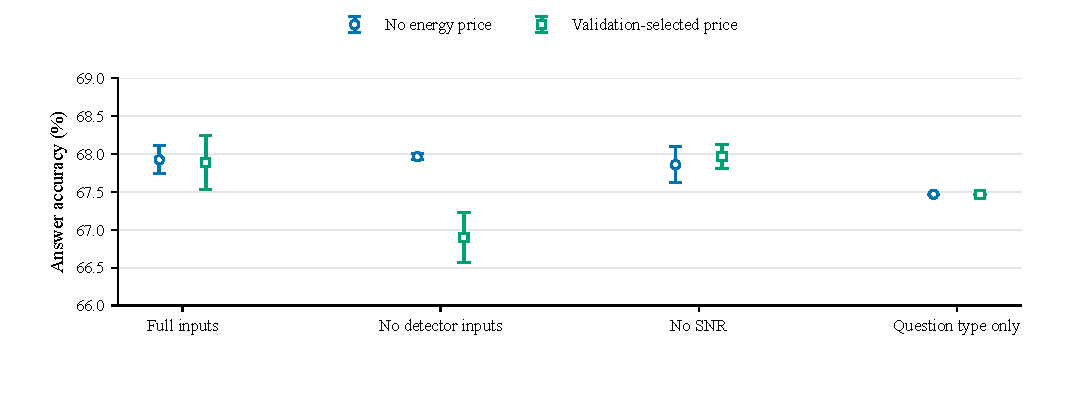
\includegraphics[width=\linewidth]{figures/evidence_final/awgn_ablation.pdf}
\caption{AWGN 输入消融：点为十种子均值，误差线为一个样本标准差。}
\end{figure}

\section{计数校准对照}
VisDrone 保留仅训练集校准和不校准对照。
AWGN 完整 MLP 在不校准时，默认准确率为 $67.36\%\pm0.18\%$，
验证选价后为 $67.22\%\pm0.30\%$。
这些结果在对应接收标签下完整重新拟合，不是事后仅更改测试答案。
DroneVehicle 的 $24$ 个类别/信噪比校准比例在训练接受规则下全部回退为 $1$，
因此三个划分的标签及对应种子的模型结果完全一致，不能视为两个独立验证。
检测器仍为 VisDrone 训练的检测器，目标数据拟合只涉及路由器。

\section{匹配接收器覆盖与适配}
\begin{table}[ht]\centering
\caption{六个信噪比点的公共测试覆盖。}
\begin{tabular}{lrr}\toprule
问题类型 & 图像数 & 决策数\\\midrule
存在性 & 26 & 624\\
计数 & 26 & 312\\
比较 & 104 & 624\\
共现 & 104 & 624\\
阈值 & 104 & 624\\
\bottomrule\end{tabular}
\end{table}
三个接收器使用相同键和接收 JPEG，但类型覆盖不均，汇总值更偏重额外三类问题。
固定同一批已拟合模型，仅评价五类齐全的 $26$ 张测试图像（$1404$ 条决策），
Qwen2、Qwen2.5、SmolVLM 的 MLP 均值为 $67.69\%$、$67.02\%$、$67.14\%$。
这些子集值作为补充，不替换正文公共键结果。
专用 MLP 的图像选择率为 $28.59\%$、$37.59\%$、$23.64\%$；
冻结 Qwen2 路由在其他接收器上保持 $28.59\%$ 的选择率，
变化的是所选目标答案的正确性，不是目标端重新选路。
替代接收器能耗没有实测，不将选择率转换成经验节能收益。

\section{变化与能耗的解释}
十种子反映固定划分上的训练变化，不是十个独立测试集。
问题、信噪比、接收器预测共享图像。
本文报告均值、样本标准差及描述性差异，不把历史 bootstrap 区间或等效检验套到修正后的策略上。
推断分析需要保持图像聚类结构并明确比较族；本文不声称统计显著或统计等效。

能耗包括建模的传输、机载检测及边缘 VLM 超空闲功率测量代理，
不包括源编码、路由、符号解码、飞行、感知和射频电路。
DroneVehicle 固定图像的无人机每题成本约 $0.132$ J，
验证选价 MLP 约 $0.450$ J；系统总成本更低主要来自边缘推理减少，
不能写成实测无人机电池收益。
